\documentclass[conference]{IEEEtran}
\IEEEoverridecommandlockouts
% The preceding line is only needed to identify funding in the first footnote. If that is unneeded, please comment it out.
\usepackage{cite}
\usepackage{amsmath,amssymb,amsfonts}
\usepackage{algorithmic}
\usepackage{graphicx}
\usepackage{textcomp}
\usepackage{graphicx}
\graphicspath{ {./images/} }
\usepackage{xcolor}
\usepackage[utf8]{inputenc}
\usepackage{hyperref}
\def\BibTeX{{\rm B\kern-.05em{\sc i\kern-.025em b}\kern-.08em
    T\kern-.1667em\lower.7ex\hbox{E}\kern-.125emX}}
\begin{document}

\title{
Largest Minimum Distance Between Two Consecutive Pairs\\
}

\author{\IEEEauthorblockN{ B. Chetan Rao}
\IEEEauthorblockA{IIB2019018}
\and
\IEEEauthorblockN{Kalpana Khutela}
\IEEEauthorblockA{IIB2019019}
\and
\IEEEauthorblockN{Devang Bharti}
\IEEEauthorblockA{IIB2019020}
}

\maketitle

\noindent \begin{abstract}

In this report we used a divide and conquer algorithm to find the largest minimum distance.and then we also calculated the time and space complexity\\\\
Keyword : longest minimum distance, space complexity, time complexity.

\end{abstract}


\section{\textbf{Introduction}}
\noindent In this problem, we have to find the largest minimum distance for given k such k<=n where n is length of array. \\\\

\noindent For example: if we have arr of 1 2 5 9 and k=2 then largest of all possible minimum distance will be 8\\

\noindent we have given a brief idea of our algorithm \textbf{part II}.\\


\section{\textbf {Algorithm Description and Analysis}}

\begin{enumerate}

\item The algorithm asks for the size of array ‘n’ as an input.\\

\item Now the algorithm asks for n integers which are now stored in an array.\\

\item Now we used the an application of divide and conquer approach named binary search to solve this problem.
\\

\item First sort the array. Maximum possible value result will be equal to a[n-1] –a[0] (for k = 2) and lower bound l = 1 and not arr[0] (because minimum distance between each element can  be one) and upper bound r = arr[n-1] (where n is the size of array arr). \\

\item We start with the middle of maximum possible result. If middle is a feasible  solution, we search on right half of mid. Else we search is left half. To check  feasibility, we place k elements under given mid-distance.
\\

\item If total number of elements found that can be placed at a minimum distance equal  to mid, is greater than or equal to k we return mid as a possible answer and  increase left = mid + 1 .
\\

\item If total number of elements found that can be placed at a minimum distance equal  to mid, is less than  k we return false and in that case right= mid-1.\\



\textbf{For Example - }


Let input be
n = 6 and k = 3 and array be: {1,2,7,5,11,12} 
 \\

After sorting the given array : {1,2,5,7,11,12}\\
Here, left = 1 and right =12\\


Applying binary search :\\\\
mid = (12+1)/2 = 6\\
Number of points possible with distance 6 equal to 2, So result = 5 and right= 6-1=5 and left = 1\\\\
mid = (5+1)/2 = 3\\
Number of points possible with distance 3 equal to 3, So left = 3 and right = 5 \\\\
mid= (3+5)/2 =4\\
Number of points possible with distance equal to 3, So left = 4 and  right = 5\\\\
Then for mid =5 number of possible points is 3 and it is the maximum possible answer.\\

We calculate the longest common prefix of the two strings, which comes out to be “Ind” and return it.\\



\end{enumerate}

\section{\textbf{Pseudo Code}} 
\noindent Function int-minimum-distance \\
Pass : int arr[ ], int n, int k\\
\begin{algorithmic}
    \STATE $sort(a)$
    \STATE $int result = -1$
    \STATE $int left = 1$
    \STATE $int result = arr[n-1]$
	\WHILE{$left < right$}
	  \STATE  $mid \gets (left+right)/2 $
	    \IF {$Is-feasible(mid,arr,n,k)$}
	      \STATE	$res = max(res,mid)$
	      \STATE	$left = mid+1$
        \ELSE
          \STATE	$right=mid$\\
return res
\end{algorithmic}

\section{\textbf{Pseudo Code II}}
\noindent Function Is-Feasible \\
Pass : int mid[ ], int arr, int n, int k\\
\begin{algorithmic}
   \STATE	$int position = arr[0]$
   \STATE	$elements = 1$
   \For{$i \gets 0$ \textbf{ to } $n$}
     \IF{$arr[i]-position >= mid$}
        \STATE $position=arr[i]$
        \STATE $elements++$
        \IF{$elements==k$}
           return 1
        \ENDIF\\
     \ENDIF
    \ENDFOR\\ 
return 0           
\end{algorithmic}


\section{\textbf {Time Complexity}}
\noindent The overall complexity of the question is O(n*log-n).
For Sorting the given array time complexity will be O(n*log-n).
Our algorithm uses binary search to find the maximum distance possible for given value of k and the complexity of binary search is O(log n).
To check the feasibility for the given value of k and mid value ,we will traverse the array .Time complexity in worst case will be O(n).
Overall time complexity = O(n*log-n)  


\begin{figure}[htp]
    \centering
    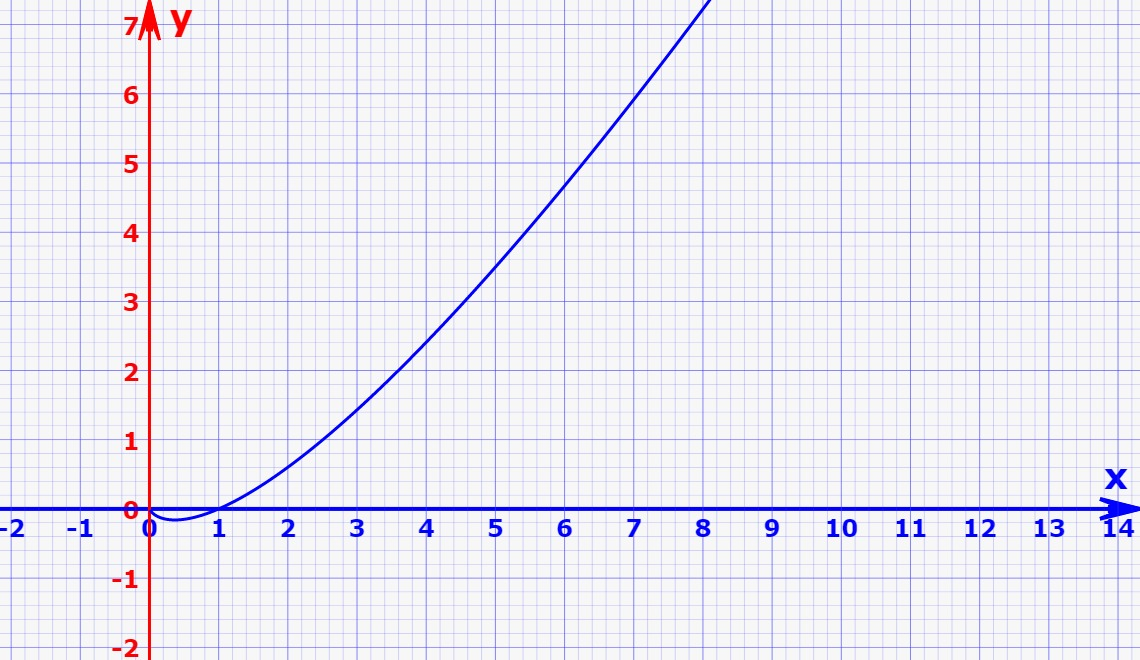
\includegraphics[width=8cm]{TimeComplexity}
    \caption{Time complexity curve}
    \label{fig:timecomplexity.png}
\end{figure}

\section{\textbf {Auxiliary Space Complexity}}
\noindent No extra space is used in this algorithm , so auxiliary space is constant.Only the input array is of size n.
Space Complexity = Input Space + Auxiliary Space ,which in turn equal to O(n).


\begin{figure}[htp]
    \centering
    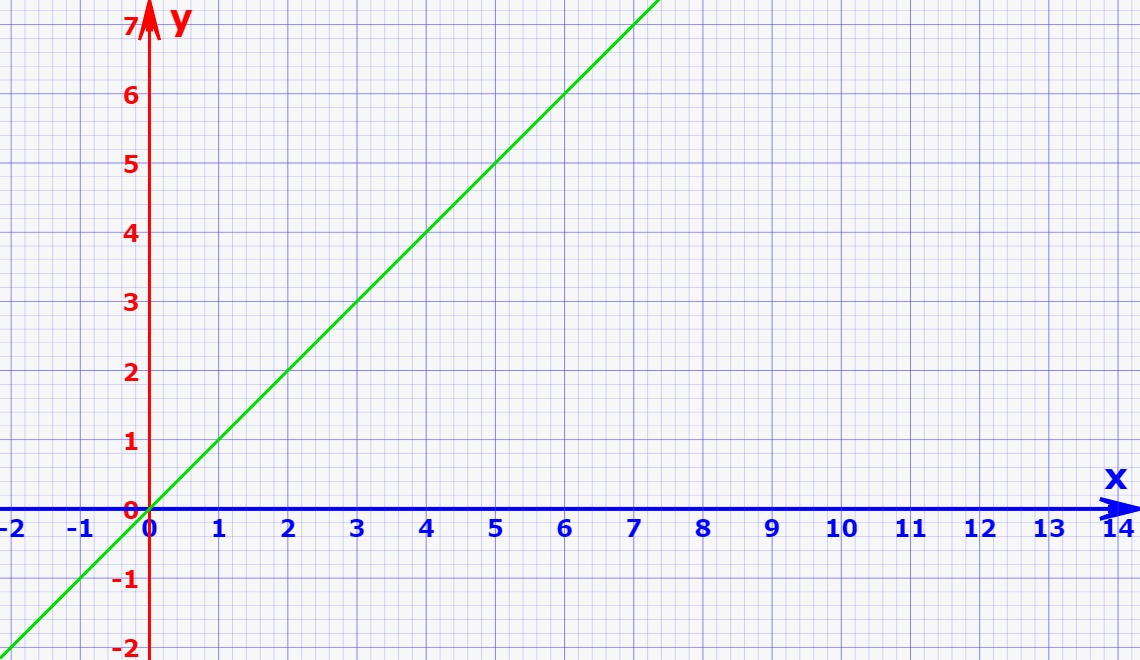
\includegraphics[width=8cm]{AuxiliarySpaceComplexity}
    \caption{Auxiliary space complexity curve}
    \label{fig:Aux.png}
\end{figure}

\section{\textbf {Conclusion}} \noindent The above proposed algorithm efficiently gives the maximum possible minimum distance  between two consecutive elements for k elements placed on given n distances on a  horizontal line. The algorithm proposed is very efficient both space and time wise with  O(n*log-n) time complexity.\\
\section{\textbf {References}} 
\begin{enumerate}

\item  \href{https://www.geeksforgeeks.org/divide-and-conquer-algorithm-introduction/}{Introduction to divide and conquer algorithm}\\
    
\item  \href{https://www.tutorialspoint.com/place-k-elements-such-that-minimum-distance-is-maximized-in-cplusplus}{
Tutorials point}
\\

\end{enumerate}

\end{document}